\documentclass[a4paper,11pt]{article}
\usepackage{hyperref}
\usepackage{graphicx}
\usepackage{listings}
\usepackage{mathabx}
\usepackage{color}

\definecolor{gray}{rgb}{0.5,0.5,0.5}

\author{Maarten Inja \and Patrick de Kok}
\title{MLPR: Lab 1}

\lstset{
  language=Octave,
  basicstyle=\footnotesize,
  numbers=left,
  numberstyle=\tiny\color{gray},
  stepnumber=5,
  showspaces=false,
  showstringspaces=true
  showtabs=false,
  frame=single,
  title=\lstname,
  breaklines=true,
}
\begin{document}
\maketitle

\section*{Exercise 1}
\begin{figure}[h]
  \caption{A plot of the dataset.  The red ``$+$'' and magenta ``$\circ$'' represent the training and test data points of class A.  The blue ``$\times$'' and black ``$\convolution$'' represent the training and test data points of class B.}
  \label{plot1}
  \begin{center}
    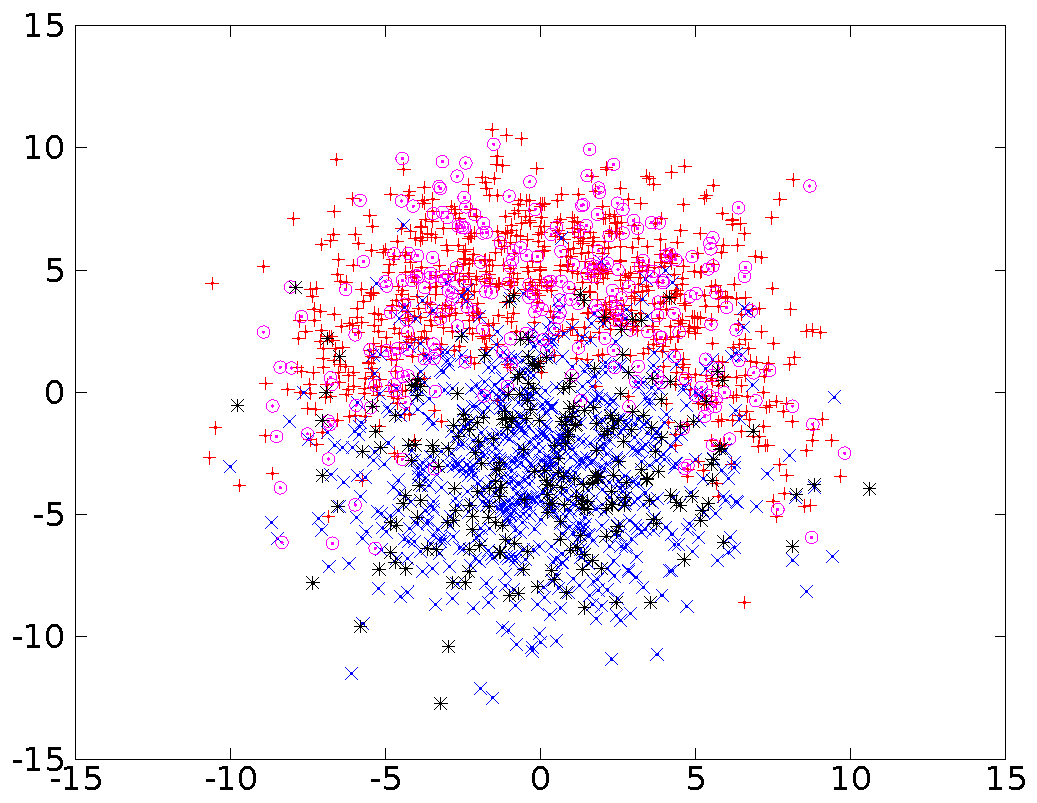
\includegraphics[width=0.6\paperwidth]{plot1}
  \end{center}
\end{figure}

Our training and test data sets are generated through the Matlab code presented in \autoref{code}.  A graphical representation is given in \autoref{plot1}.

\lstinputlisting[caption={The code which generates our data set},label=code]{preprocess_data.m}

\section*{Exercise 2}
Confusion matrices of the KNN with $1 \leq k \leq 20$:

\begin{table}
  \caption{TA = True A; TB = True B; CA = classified as A; CB = classified as B.}
\begin{tabular}{lcrr}
$k$ && CA & CB \\ \\
 1 & TA & 199 &    51 \\
& TB &  34 &   216 \\
 2 & TA & 205 &    45 \\
& TB &  34 &   216 \\
 3 & TA & 212 &    38 \\
& TB &  33 &   217 \\
 4 & TA & 217 &    33 \\
& TB &  35 &   215 \\
 5 & TA & 214 &    36 \\
& TB &  30 &   220 \\
 6 & TA & 217 &    33 \\
& TB &  31 &   219 \\
 7 & TA & 216 &    34 \\
& TB &  31 &   219 \\
 8 & TA & 221 &    29 \\
& TB &  32 &   218 \\
 9 & TA & 216 &    34 \\
& TB &  30 &   220 \\
 10 & TA & 217 &    33 \\
& TB &  32 &   218 \\
 11 & TA & 214 &    36 \\
& TB &  29 &   221 \\
 12 & TA & 215 &    35 \\
& TB &  28 &   222 \\
 13 & TA & 215 &    35 \\
& TB &  31 &   219 \\
 14 & TA & 216 &    34 \\
& TB &  31 &   219 \\
 15 & TA & 216 &    34 \\
& TB &  31 &   219 \\
 16 & TA & 213 &    37 \\
& TB &  31 &   219 \\
 17 & TA & 215 &    35 \\
& TB &  35 &   215 \\
 18 & TA & 215 &    35 \\
& TB &  34 &   216 \\
 19 & TA & 215 &    35 \\
& TB &  36 &   214 \\
 20 & TA & 216 &    34 \\
& TB &  33 &   217 \\
\end{tabular}
\end{table}

\section*{Exercise 3}

\end{document}
